\documentclass[border=2mm,12pt,tikz]{standalone}
\usepackage{tikz-3dplot} 
\usepackage{bm}
\usetikzlibrary{intersections,patterns.meta}
\begin{document}
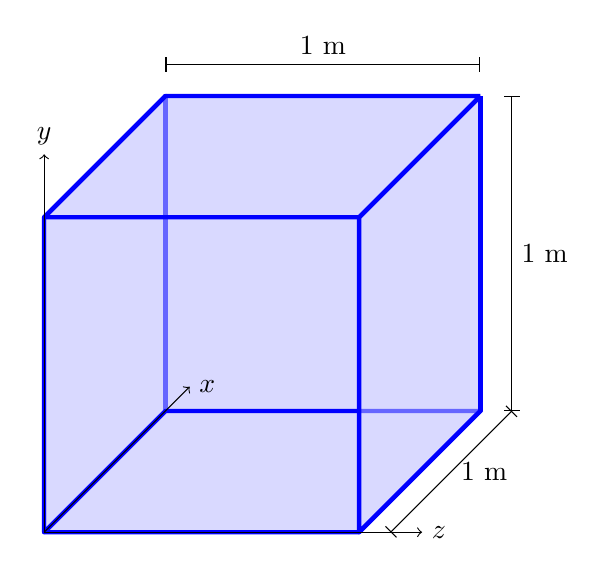
\begin{tikzpicture}[
        scale = 4, 
        line join=round,
        mystyle/.style = {ultra thick, blue, fill=blue!20, fill opacity=0.5},
        rotate around y=90
    ]

    \coordinate (1) at (1, 1, 1);
    \coordinate (2) at (1, 0, 1);
    \coordinate (3) at (1, 0, 0);
    \coordinate (4) at (1, 1, 0);
    \coordinate (5) at (0, 0, 1);
    \coordinate (6) at (0, 0, 0);
    \coordinate (7) at (0, 1, 0);
    \coordinate (8) at (0, 1, 1);

    \draw[mystyle] (3) -- (4) -- (7) -- (6) -- (3);
    \draw[mystyle] (1) -- (2) -- (3) -- (4) -- (1);
    \draw[mystyle] (5) -- (6) -- (7) -- (8) -- (5);
    \draw[mystyle] (1) -- (4) -- (7) -- (8) -- (1);
    \draw[mystyle] (2) -- (3) -- (6) -- (5) -- (2);
    \draw[mystyle] (1) -- (2) -- (5) -- (8) -- (1);

    \draw[->] (0, 0, 0) -- (1.2, 0, 0) node[right] {$x$};
    \draw[->] (0, 0, 0) -- (0, 1.2, 0) node[above] {$y$};
    \draw[->] (0, 0, 0) -- (0, 0, 1.2) node[right] {$z$};

    \draw[|-|] (4) ++ (0, 0.1, 0) --++ (0,0,1) node[midway, above] {$1$ m};
    \draw[|-|] (2) ++ (0, 0, 0.1) --++ (0,1,0) node[midway, right] {$1$ m};
    \draw[|-|] (5) ++ (0, 0, 0.1) --++ (1,0,0) node[midway, right] {$1$ m};
\end{tikzpicture}
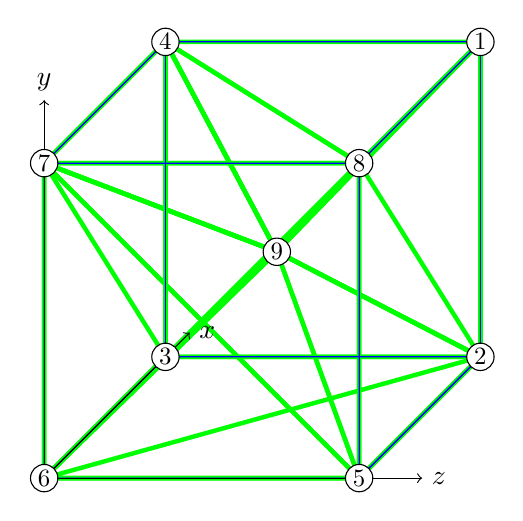
\begin{tikzpicture}[
        scale = 4, 
        line join=round,
        mystyle/.style = {ultra thick, green},
        mystyle2/.style = {blue},
        rotate around y=90
    ]
        \coordinate (1) at (1, 1, 1);
        \coordinate (2) at (1, 0, 1);
        \coordinate (3) at (1, 0, 0);
        \coordinate (4) at (1, 1, 0);
        \coordinate (5) at (0, 0, 1);
        \coordinate (6) at (0, 0, 0);
        \coordinate (7) at (0, 1, 0);
        \coordinate (8) at (0, 1, 1);
        \coordinate (9) at (0.49, 0.53, 0.55);

        \draw[mystyle] (2) -- (6) -- (5) -- (9) -- cycle;
        \draw[mystyle] (9) -- (6) -- (5) -- (7) -- cycle;
        \draw[mystyle] (7) -- (9) -- (8) -- (5) -- cycle;
        \draw[mystyle] (6) -- (7) -- (9) -- (3) -- cycle;
        \draw[mystyle] (4) -- (9) -- (1) -- (8) -- cycle;
        \draw[mystyle] (3) -- (4) -- (9) -- (1) -- cycle;
        \draw[mystyle] (3) -- (7) -- (9) -- (4) -- cycle;
        \draw[mystyle] (3) -- (9) -- (2) -- (1) -- cycle;
        \draw[mystyle] (5) -- (9) -- (8) -- (2) -- cycle;
        \draw[mystyle] (9) -- (2) -- (1) -- (8) -- cycle;
        \draw[mystyle] (6) -- (9) -- (2) -- (3) -- cycle;
        \draw[mystyle] (7) -- (9) -- (4) -- (8) -- cycle;
          
        \draw[mystyle] (3) -- (4) -- (7) -- (6) -- (3);
        \draw[mystyle] (1) -- (2) -- (3) -- (4) -- (1);
        \draw[mystyle] (5) -- (6) -- (7) -- (8) -- (5);
        \draw[mystyle] (1) -- (4) -- (7) -- (8) -- (1);
        \draw[mystyle] (2) -- (3) -- (6) -- (5) -- (2);
        \draw[mystyle] (1) -- (2) -- (5) -- (8) -- (1);
        
        \draw[mystyle2] (3) -- (4) -- (7) -- (6) -- (3);
        \draw[mystyle2] (1) -- (2) -- (3) -- (4) -- (1);
        \draw[mystyle2] (5) -- (6) -- (7) -- (8) -- (5);
        \draw[mystyle2] (1) -- (4) -- (7) -- (8) -- (1);
        \draw[mystyle2] (2) -- (3) -- (6) -- (5) -- (2);
        \draw[mystyle2] (1) -- (2) -- (5) -- (8) -- (1);

        \draw[->] (0, 0, 0) -- (1.2, 0, 0) node[right] {$x$};
        \draw[->] (0, 0, 0) -- (0, 1.2, 0) node[above] {$y$};
        \draw[->] (0, 0, 0) -- (0, 0, 1.2) node[right] {$z$};

        \draw (1) node[ circle, draw, inner sep=1pt, fill=white, thin, scale = 0.9, fill opacity = 1] {$1$};
        \draw (2) node[ circle, draw, inner sep=1pt, fill=white, thin, scale = 0.9, fill opacity = 1] {$2$};
        \draw (3) node[ circle, draw, inner sep=1pt, fill=white, thin, scale = 0.9, fill opacity = 1] {$3$};
        \draw (4) node[ circle, draw, inner sep=1pt, fill=white, thin, scale = 0.9, fill opacity = 1] {$4$};
        \draw (5) node[ circle, draw, inner sep=1pt, fill=white, thin, scale = 0.9, fill opacity = 1] {$5$};
        \draw (6) node[ circle, draw, inner sep=1pt, fill=white, thin, scale = 0.9, fill opacity = 1] {$6$};
        \draw (7) node[ circle, draw, inner sep=1pt, fill=white, thin, scale = 0.9, fill opacity = 1] {$7$};
        \draw (8) node[ circle, draw, inner sep=1pt, fill=white, thin, scale = 0.9, fill opacity = 1] {$8$};
        \draw (9) node[ circle, draw, inner sep=1pt, fill=white, thin, scale = 0.9, fill opacity = 1] {$9$};

    \end{tikzpicture}
    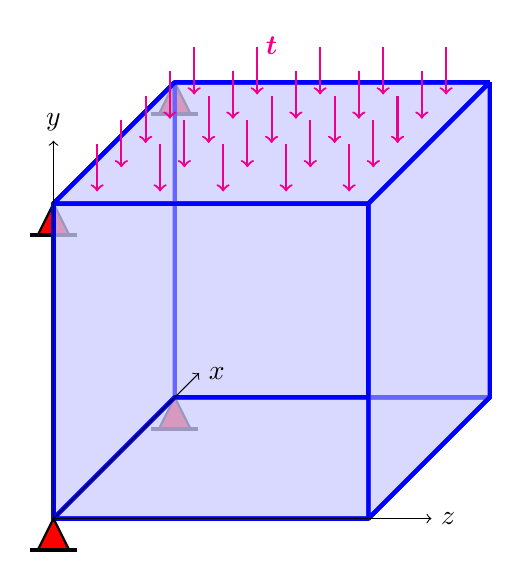
\begin{tikzpicture}[
        scale = 4, 
        line join=round,
        mystyle/.style = {ultra thick, blue, fill=blue!20, fill opacity=0.5},
        rotate around y=90
    ]

    \coordinate (1) at (1, 1, 1);
    \coordinate (2) at (1, 0, 1);
    \coordinate (3) at (1, 0, 0);
    \coordinate (4) at (1, 1, 0);
    \coordinate (5) at (0, 0, 1);
    \coordinate (6) at (0, 0, 0);
    \coordinate (7) at (0, 1, 0);
    \coordinate (8) at (0, 1, 1);

    \draw[thick, fill = red] (4) --++ (0, -0.1, 0.05) --++ (0, 0, -0.1) -- cycle;
    \draw[ultra thick] (4) ++ (0, -0.1, 0.075) --++ (0, 0, -0.15);

    \draw[thick, fill = red] (3) --++ (0, -0.1, 0.05) --++ (0, 0, -0.1) -- cycle;
    \draw[ultra thick] (3) ++ (0, -0.1, 0.075) --++ (0, 0, -0.15);

    \draw[thick, fill = red] (7) --++ (0, -0.1, 0.05) --++ (0, 0, -0.1) -- cycle;
    \draw[ultra thick] (7) ++ (0, -0.1, 0.075) --++ (0, 0, -0.15);

    \draw[mystyle] (3) -- (4) -- (7) -- (6) -- (3);
    \draw[mystyle] (1) -- (2) -- (3) -- (4) -- (1);
    \draw[mystyle] (5) -- (6) -- (7) -- (8) -- (5);
    \draw[mystyle] (1) -- (4) -- (7) -- (8) -- (1);
    \draw[mystyle] (2) -- (3) -- (6) -- (5) -- (2);
    \draw[mystyle] (1) -- (2) -- (5) -- (8) -- (1);

    \draw[->] (0, 0, 0) -- (1.2, 0, 0) node[right] {$x$};
    \draw[->] (0, 0, 0) -- (0, 1.2, 0) node[above] {$y$};
    \draw[->] (0, 0, 0) -- (0, 0, 1.2) node[right] {$z$};

    \draw[thick, fill = red] (6) --++ (0, -0.1, 0.05) --++ (0, 0, -0.1) -- cycle;
    \draw[ultra thick] (6) ++ (0, -0.1, 0.075) --++ (0, 0, -0.15);


    \foreach \z in {0.1, 0.3, ..., 0.9} {
        \foreach \x in {0.1, 0.3, ..., 0.9} {
            \draw[<-, magenta, thick] (\x, 1, \z) --++ (0, 0.15, 0);
        }
    }

    \draw (0.5, 1.25, 0.5) node[above, magenta] {$\bm{t}$};

\end{tikzpicture}
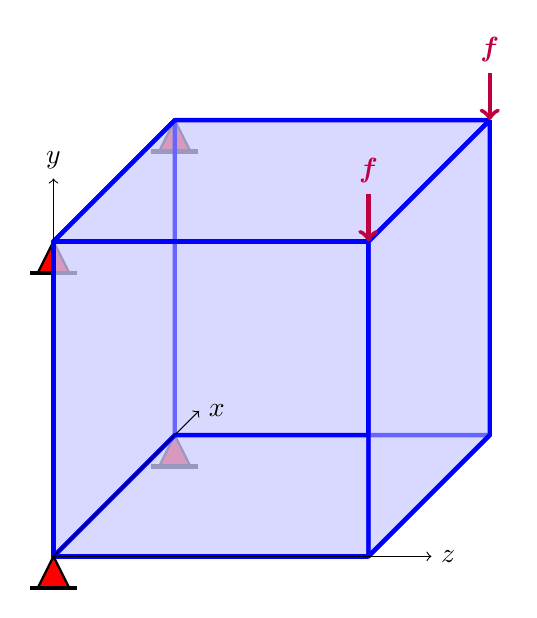
\begin{tikzpicture}[
    scale = 4, 
    line join=round,
    mystyle/.style = {ultra thick, blue, fill=blue!20, fill opacity=0.5},
    rotate around y=90
]

\coordinate (1) at (1, 1, 1);
\coordinate (2) at (1, 0, 1);
\coordinate (3) at (1, 0, 0);
\coordinate (4) at (1, 1, 0);
\coordinate (5) at (0, 0, 1);
\coordinate (6) at (0, 0, 0);
\coordinate (7) at (0, 1, 0);
\coordinate (8) at (0, 1, 1);

\draw[thick, fill = red] (4) --++ (0, -0.1, 0.05) --++ (0, 0, -0.1) -- cycle;
\draw[ultra thick] (4) ++ (0, -0.1, 0.075) --++ (0, 0, -0.15);

\draw[thick, fill = red] (3) --++ (0, -0.1, 0.05) --++ (0, 0, -0.1) -- cycle;
\draw[ultra thick] (3) ++ (0, -0.1, 0.075) --++ (0, 0, -0.15);

\draw[thick, fill = red] (7) --++ (0, -0.1, 0.05) --++ (0, 0, -0.1) -- cycle;
\draw[ultra thick] (7) ++ (0, -0.1, 0.075) --++ (0, 0, -0.15);

\draw[mystyle] (3) -- (4) -- (7) -- (6) -- (3);
\draw[mystyle] (1) -- (2) -- (3) -- (4) -- (1);
\draw[mystyle] (5) -- (6) -- (7) -- (8) -- (5);
\draw[mystyle] (1) -- (4) -- (7) -- (8) -- (1);
\draw[mystyle] (2) -- (3) -- (6) -- (5) -- (2);
\draw[mystyle] (1) -- (2) -- (5) -- (8) -- (1);

\draw[->] (0, 0, 0) -- (1.2, 0, 0) node[right] {$x$};
\draw[->] (0, 0, 0) -- (0, 1.2, 0) node[above] {$y$};
\draw[->] (0, 0, 0) -- (0, 0, 1.2) node[right] {$z$};

\draw[thick, fill = red] (6) --++ (0, -0.1, 0.05) --++ (0, 0, -0.1) -- cycle;
\draw[ultra thick] (6) ++ (0, -0.1, 0.075) --++ (0, 0, -0.15);



\draw[<-, ultra thick, purple] (8) --++ (0,0.15,0) node[above, purple] {$\bm{f}$};
\draw[<-, ultra thick, purple] (1) --++ (0,0.15,0) node[above, purple] {$\bm{f}$};

\end{tikzpicture}
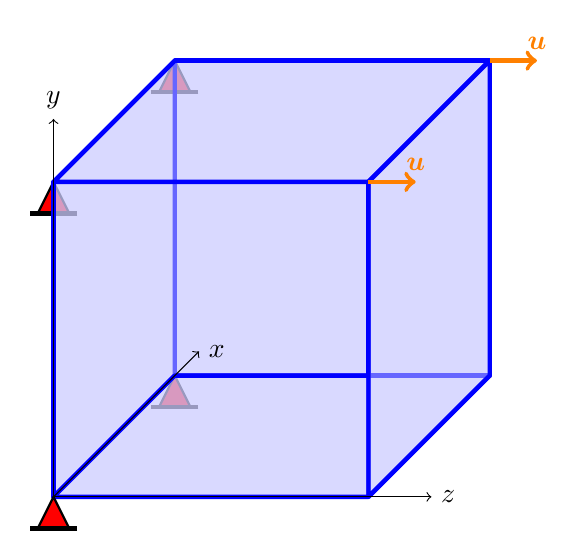
\begin{tikzpicture}[
    scale = 4, 
    line join=round,
    mystyle/.style = {ultra thick, blue, fill=blue!20, fill opacity=0.5},
    rotate around y=90
]

\coordinate (1) at (1, 1, 1);
\coordinate (2) at (1, 0, 1);
\coordinate (3) at (1, 0, 0);
\coordinate (4) at (1, 1, 0);
\coordinate (5) at (0, 0, 1);
\coordinate (6) at (0, 0, 0);
\coordinate (7) at (0, 1, 0);
\coordinate (8) at (0, 1, 1);

\draw[thick, fill = red] (4) --++ (0, -0.1, 0.05) --++ (0, 0, -0.1) -- cycle;
\draw[ultra thick] (4) ++ (0, -0.1, 0.075) --++ (0, 0, -0.15);

\draw[thick, fill = red] (3) --++ (0, -0.1, 0.05) --++ (0, 0, -0.1) -- cycle;
\draw[ultra thick] (3) ++ (0, -0.1, 0.075) --++ (0, 0, -0.15);

\draw[thick, fill = red] (7) --++ (0, -0.1, 0.05) --++ (0, 0, -0.1) -- cycle;
\draw[ultra thick] (7) ++ (0, -0.1, 0.075) --++ (0, 0, -0.15);

\draw[mystyle] (3) -- (4) -- (7) -- (6) -- (3);
\draw[mystyle] (1) -- (2) -- (3) -- (4) -- (1);
\draw[mystyle] (5) -- (6) -- (7) -- (8) -- (5);
\draw[mystyle] (1) -- (4) -- (7) -- (8) -- (1);
\draw[mystyle] (2) -- (3) -- (6) -- (5) -- (2);
\draw[mystyle] (1) -- (2) -- (5) -- (8) -- (1);

\draw[->] (0, 0, 0) -- (1.2, 0, 0) node[right] {$x$};
\draw[->] (0, 0, 0) -- (0, 1.2, 0) node[above] {$y$};
\draw[->] (0, 0, 0) -- (0, 0, 1.2) node[right] {$z$};

\draw[thick, fill = red] (6) --++ (0, -0.1, 0.05) --++ (0, 0, -0.1) -- cycle;
\draw[ultra thick] (6) ++ (0, -0.1, 0.075) --++ (0, 0, -0.15);



\draw[->, ultra thick, orange] (8) --++ (0,0,0.15) node[above, orange] {$\bm{u}$};
\draw[->, ultra thick, orange] (1) --++ (0,0,0.15) node[above, orange] {$\bm{u}$};

\end{tikzpicture}
\end{document} 